
Для разрешения проблемы долгосрочного планирования предложено 
использовать ассистента совместно с рекомендационную систему,
выполняющую задачи поиска задачи оптимальной сложности и .

Большие языковые модели не гарантируют корректное исполнение даже базовых арифметических операций сложения . 
В обзоре \cite{zhao2023survey} показано, что подобные проблемы возникают во многих строгих постановках, где
соблюдение формы требует интеллектуального участия: написание исполняемого языком программирования кода,
переход в математических выражениях.

Для разрешения проблемы исследователи предложили использование инструментов,
которые используются моделью для качественного выполнения инструкции. На данный момент сложились \begin{itemize}
    \item обращения к информационным системам  (RAG - retreival augmented generation)\cite{lewis2020retrieval}
    \item работа с средой исполнения программного кода \cite{parisi2022talm}
    \item генерация сопровождающей иллюстрации
\end{itemize}

Направление имеет большие перспективы, использование.

Тем не менее современные модели пока 



\begin{figure}[h]
    \centering
    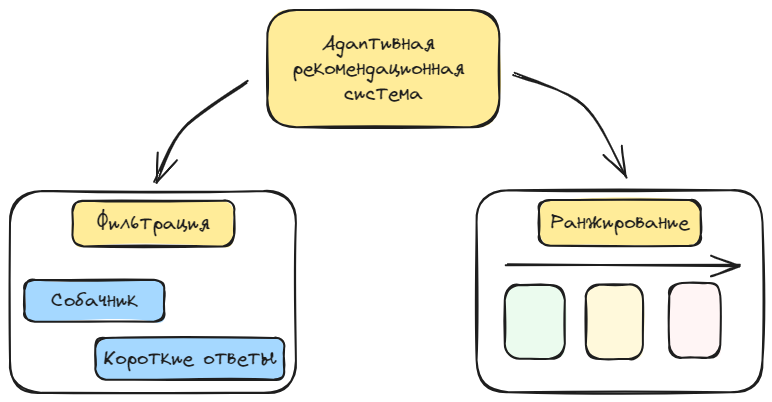
\includegraphics[width=0.5\textwidth]{assets/work/rating/bayes.excalidraw.png}
    \caption{Ht}
    \label{recommendation}
\end{figure}

Подход совмещающий использование ассистента совместно.
Существуют постановки, в которых вызов инструментов выполняется 

Таким образом, итоговый ассистент с
Совмещающий байесову рекомендательную систему как систему долгосрочного планирования и ассистента как эмпатического посредника.


\begin{figure}[h]
    \centering
    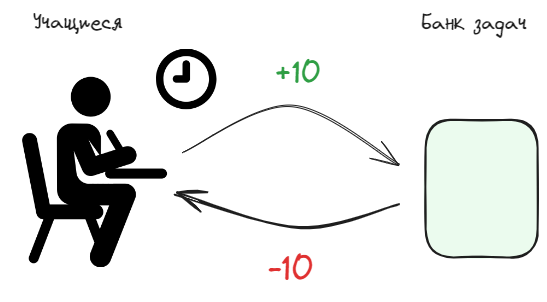
\includegraphics[width=0.5\textwidth]{assets/work/rating/recommendation.excalidraw.png}
    \caption{Проект приложения}
    \label{arch}
\end{figure}

Байесовы рейтинговые модели задают правила обновления апостериорных представлений рейтинга. Наиболее известным примером байесовой модели рейтинга является модель Брэдли-Терри и эквивалентная ей модель Эло.

Ключевым преимуществом байесовых систем является возможность пересчета рейтинга сразу после матча. Таким образом система приобретает адаптивность, важную в коммуникациях в настоящем времени.






В такой постановке ассистент следит за эмоциональным откликом обучающегося на материал,
узнает ее причину и в случае несоразмерной уровню нагрузке сообщает управляющей системе о потребности изменения сложности.

Плюсами такого подхода является \begin{itemize}
    \item интерпретируемость
    \item сужение ассистента до строгой постановки поиска наилучших навыков общения исходя из A/B тестирования.
\end{itemize}



